\chapter{Implémentation}

\section{Introduction}

Dans ce chapitre, on va implémenter les modèles qu'on a décri dans le chapitre précédent tout en suivant les paradigme que Keras et Larq respectent.
\paragraph{Définition des types}
Bien que Python est dynamiquement typé, nous allons inférer dans ce chapitre et dans notre bibliothèque un typage statique pour faciliter la compréhension.
\newline Nous allons dénoter pour un ensemble de types $T,T_1,\dots,T_n,Q,Q_1,\dots,Q_m$:
\begin{itemize}
	\item $\texttt{List}[T]$ pour n'importe quel itérable sur $T$
	\item $\texttt{Tuple}[T_1,\dots,T_n]$ pour un tuple contenant  des éléments de $T_1,\dots,T_n$ dans l'ordre indiqué.
	\item $\mathcal{T}[T]=\texttt{Tensor}[T]$  pour un type compatible avec 	\texttt{tensorflow.Tensor} avec \texttt{dtype}=$T$
	\item $\mathcal{T}[T,n]=\texttt{Tensor}[T,n]$  pour un type compatible avec 	\texttt{tensorflow.Tensor} avec un rang égal à $n$ et avec \texttt{dtype}=$T$
	\item $\mathcal{V}[T]=\texttt{Vector}[T]$ pour un type compatible avec 	\texttt{tensorflow.Tensor} avec un rang égal à $1$ et avec \texttt{dtype}=$T$
	\item $\mathcal{M}[T]=\texttt{Matrix}[T]$  pour un type compatible avec 	\texttt{tensorflow.Tensor} avec un rang égal à $2$ et avec \texttt{dtype}=$T$
	\item $\mathcal{R}[T]=\texttt{Random}[T]$ pour une fonction aléatoire sans arguments.
	\item $\mathcal{F}[T_1,\dots,T_n\rightarrow Q_1,\dots,Q_m]=\texttt{Function}[T_1,\dots,T_n\rightarrow Q_1,\dots,Q_m]$ pour une fonction dont les arguments sont de types respectifs $T_1,\dots,T_n$ et dont les valeurs sonts de types respectifs $Q_1,\dots,Q_m$
	\item $\End[T]=\texttt{Function}[T_1,\dots,T_n\rightarrow T_1,\dots,T_n]$ pour une fonction dont l'argument et les valeurs sont de types respectifs $T_1,\dots,T_n$. 
	\item $\mathcal{P}[T_1,\dots,T_n]=\texttt{Predicate}[T_1,\dots,T_n]$ pour un prédicat (fonction booléenne)  acceptant $n$ arguments de types respectifs $T_1,\dots,T_n$
\end{itemize}
\newpage
\section{Paradigmes}
\subsection{Dans l'implémentation de BinaryFlow}\label{Paradigm:Implementation}
Dans l'implémentations de la bibliothèque BinaryFlow, nous avons adopté principalement:
\begin{itemize}
	\item La programmation orientée objet
	\item La programmation générique
\end{itemize}
\subsubsection{Programmation orientée objet}

\subsubsection{Programmation générique}

\subsection{Dans l'utilisation de BinaryFlow}\label{Paradigm:User}
Etant une extension de Keras et Larq, nous recommenderions l'utilisateur à suivre les bonnes pratiques de ces bibliothèques.
\newline En effet nous encouragerions à suivre une de ces interfaces:
\begin{itemize}
	\item L'interface Séquentielle
	\item L'interface fonctionnelle
	\item L'interface orientée objet
\end{itemize}
\subsubsection{Interface séquentielle}
C'est l'interface la plus facile à exploiter, mais naturellement elle ne supporte pas les couches résiduales.
\newline L'utilisation de cette interface sert à créer une objet de type \texttt{tensorflow.keras.Sequential} contenant la séquence des couches dont le type est \texttt{List[tensorflow.keras.layers.Layer]}


\subsubsection{Interface fonctionnelle}
Cette interface met en valeur le fait qu'un modèle se traduit en des fonctions évaluer dans un certian ordre à un tenseur initial $X$.
\newline Pour cela, cette interface introduit un tenseur symbolique $\boldsymbol{X}$ qui décrit l'entrée du réseau de neurones. Puis les fonctions sont appliqués au tenseur $\boldsymbol{X}$ pour établir le modèle et fixer les dimensions de:
\begin{itemize}
	\item Ces paramètres
	\item L'entrée de chaque fonction
	\item La sortie de chaque fonction
\end{itemize}
Une fois le modèle est construit, on peut l'entraîner, et puis le déployer.

\subsubsection{Interface orientée objet}
Cette interface met en valeur l'aspect orienté objet de TensorFlow (et aussi BinaryFlow), il se base sur le faite qu'un utilisateur peut définir son modèle en héritant de la classe \texttt{tensorflow.keras.Model}
\newline En utilisant cette interface, l'utilisateur peut surcharger les méthodes de \texttt{tensorflow.keras.Model}, ce qui lui permet de personnaliser:
\begin{itemize}
	\item L'entraînement du modèle
	\item L'inférence du modèle
	\item L'évaluation du modèle
	\item La fonction coût du modèle
	\item ...
\end{itemize}

\subsubsection{Interface bas niveaux}
Cette interface utilise directement les fonctionnalités de TensorFlow sans exploiter Keras. Elle est aussi supportée par BinaryFlow, mais on ne la recommende que pour les utilisateurs avancés.

\subsection{Dans l'extension de BinaryFlow}
Pour éténdre notre bibliothèques, nous recommenderions de suivre les paradigmes utilisées dans l'implémentation qui sont décrite dans la section \ref{Paradigm:Implementation}.

\section{Conception}
BinaryFlow est implémentés sous formes des modules suivants:
\begin{itemize}
	\item Module des couches
	\item Module des blocs
	\item Module des quantificateurs
	\item Module des coûts
\end{itemize}

\begin{figure}[htp]
	\centering
	\begin{tikzpicture}
	\begin {package}{binaryflow}
		\begin {class}[text width=3cm]{layers}{0 ,0}
		\end{class}
		\begin {class}[text width=3cm]{blocs}{0 ,2cm}
		\end{class}
		\begin {class}[text width=3cm]{quantizers}{5cm ,0}
		\end{class}
		\begin {class}[text width=3cm]{losses}{5cm ,2cm}
		\end{class}
	\end{package}
	\end{tikzpicture}
	\caption{Structure de la bibliothèque}
\end{figure}


Dans les sections suivantes nous allons parler de chaque module.
\section{Couches}
Ce module est l'implémentation des couches des modèles suivant:
\begin{itemize}
	\item BinaryNet
	\item XnorNet
	\item ABCNet
\end{itemize}
Dans ce module, chaque couche admet un nom de la forme \texttt{NomModèle.TypeCouche} avec:
\begin{itemize}
	\item $\texttt{NomModèle} \in \{\texttt{BinaryNet},\texttt{XnorNet},\texttt{ABCNet}\}$
	\item $\texttt{TypeCouche} \in \{\texttt{Dense},\texttt{Conv1D},\texttt{Conv2D},\texttt{Conv3D}\}$
\end{itemize} 

\begin{figure}[htp]
	\small
	\centering
	\begin{tikzpicture}
		\begin {package}{layers}
			\begin {class}[text width= 3cm]{BinaryNet}{0, 0}
			\attribute{Dense}
			\attribute{Conv1D}
			\attribute{Conv2D}
			\attribute{Conv3D}
			\end{class}
			\begin {class}[text width= 3cm]{XnorNet}{4cm ,0cm}
						\attribute{Dense}
			\attribute{Conv1D}
			\attribute{Conv2D}
			\attribute{Conv3D}
			\end{class}
			\begin {class}[text width= 3cm]{ABCNet}{8cm ,0cm}
						\attribute{Dense}
			\attribute{Conv1D}
			\attribute{Conv2D}
			\attribute{Conv3D}
			\end{class}
		\end{package}
	\end{tikzpicture}
	\caption{Le contenu de \texttt{layers}}
\end{figure}
\FloatBarrier
\newpage
\subsection{BinaryNet}\label{BinaryNet:Module}
Le module \texttt{BinaryNet} contient $4$ classes qui sont: \texttt{Dense},\texttt{Conv1D},\texttt{Conv2D} et \texttt{Conv3D}.
Nous avons définir ces classes comme des synonymes respectivement de \texttt{Larq.layers.QuantDense},\texttt{Larq.layers.QuantConv1D},\texttt{Larq.layers.QuantConv2D} et \texttt{Larq.layers.QuantConv3D}
\subsubsection{API commun}
Ces $4$ couches admettent des attributs similaires, qui sont:
\begin{itemize}
	\item \texttt{kernel\_quantizer} qui est la quantification de poids.
	\item \texttt{input\_quantizer} qui est la quantification des noeuds. 
	\item \texttt{kernel\_constraint} qui est la contrainte sur les poids.
\end{itemize}
Pour conformer à la formulation originale de BinaryNet \cite{BinaryNetPaper} et BinaryConnect \cite{BinaryConnectPaper} ces valeurs doivent être initialisés à 

\begin{table}[ht]
	\centering
	\begin{tabularx}{\textwidth}{| p{3.5cm} | X |}
		\hline
		Attribut & Valeur \\
		\hline
		 \texttt{kernel\_quantizer} & \begin{itemize}
		 	\item \texttt{Larq.quantizers.SteSign}
		 	\item \texttt{BinaryFlow.quantizers.StochasticSteSign}
		 \end{itemize}  \\ 
		\hline
		\texttt{input\_quantizer} & \begin{itemize}
			\item \texttt{Larq.quantizers.SteSign}
			\item \texttt{BinaryFlow.quantizers.StochasticSteSign}
		\end{itemize}  \\ 
		\hline 
		\texttt{kernel\_constraint} & \begin{itemize}
			\item \texttt{weight\_clip}
		\end{itemize}  \\ 
		\hline
	\end{tabularx}
	\caption{Terminologie de la division en Lots}
	\label{table:BinaryNetInitialisation}
\end{table}
\FloatBarrier
\subsubsection{Dense}
Les attributs définissant cette couches sont:
\begin{itemize}
	\item \texttt{units} qui est la dimension de sortie
	\item \texttt{kernel} qui est la matrice de paramètres
\end{itemize}
\subsubsection{ConvND}
Les couches convolutionnelles admettent des attributs similaires.
\newline Pour une couche convolutionnelle à $N\in\{1,2,3\}$ dimensions, on a:
\begin{itemize}
	\item \texttt{filters} est le nombre de canaux de sorties.
	\item \texttt{kernel\_size} est la taille du noyau de convolution
	\item \texttt{padding} est le padding utilisée dans la convolution.
	\item \texttt{strides} est la taille de pas entre deux convolutions successives
\end{itemize} 
\begin{figure}[htp]
	\small
	\begin{tikzpicture}
		\begin {package}{BinaryNet}
		\begin {class}[text width= 7cm ]{Dense}{0, 0}
		\attribute{units : int}
		\attribute{kernel : Matrix[float]}
		\attribute{kernel\_qunatizer : $\End[\mathcal{T}[\texttt{float}]]$}
		\attribute{input\_quantizer : $\End[\mathcal{T}[\texttt{float}]]$}
		\attribute{kernel\_constraint : Predicate[Matrix[float]]}
		\vdots
	\end{class}
	\begin {class}[text width= 7cm ]{Conv1D}{0 ,6cm}
	\attribute{filters : int}
	\attribute{kernel\_size : int}
	\attribute{kernel : Vector[float]}
	\attribute{strides : int}
	\attribute{padding}
	\attribute{kernel\_qunatizer : $\End[\mathcal{T}[\texttt{float}]]$}
	\attribute{input\_quantizer : $\End[\mathcal{T}[\texttt{float}]]$}
	\attribute{kernel\_constraint : Predicate[Matrix[float]]}
	\attribute{\vdots}
	\end{class}
	\begin {class}[text width= 7cm ]{Conv2D}{8cm ,0}
	\attribute{filters : int}
	\attribute{kernel\_size : Tuple[int,int]}
	\attribute{kernel : Matrix[float]}
	\attribute{strides : int}
	\attribute{padding}
	\attribute{kernel\_qunatizer : $\End[\mathcal{T}[\texttt{float}]]$}
	\attribute{input\_quantizer : $\End[\mathcal{T}[\texttt{float}]]$}
	\attribute{kernel\_constraint : Predicate[Matrix[float]]}
	\attribute{\vdots}
	\end{class}
	\begin {class}[text width= 7cm ]{Conv3D}{8cm ,6cm}
	\attribute{filters : int}
	\attribute{kernel\_size : Tuple[int,int,int]}
	\attribute{kernel : Tensor[float,float,float]}
	\attribute{strides : int}
	\attribute{padding}
	\attribute{kernel\_qunatizer : $\End[\mathcal{T}[\texttt{float}]]$}
	\attribute{input\_quantizer : $\End[\mathcal{T}[\texttt{float}]]$}
	\attribute{kernel\_constraint : Predicate[Matrix[float]]}
	\attribute{\vdots}
	\end{class}
	\end{package}
\end{tikzpicture}
\caption{BinaryNet}
\end{figure}
\FloatBarrier
\newpage 
\subsection{XnorNet}
Le module \texttt{XnorNet} contient $4$ classes qui sont: \texttt{Dense},\texttt{Conv1D},\texttt{Conv2D} et \texttt{Conv3D}.
\newline Chacune de ces classes est une classe fille de son contrepart dans le module \texttt{BinaryNet} présenté dans \ref{BinaryNet:Module}. 
\subsubsection{Attributs Ajouté}
Le seul attribut ajouté est \texttt{alpha\_trainable} qui demande si $\alpha$ doit être entrainé ou non. Par défaut il est égal à \texttt{False}.
\subsubsection{Initialisaiton de $\alpha$}
Indépendemment de \texttt{alpha\_trainable}, $\alpha$ est toujours initialisé à \ref{XnorNet:FullyConnected} dans le cas d'une couche dense, et à \ref{XnorNet:FullyConnected} dans le cas d'une couche convolutionnelle.
\begin{figure}[htp]
	\small
	\begin{tikzpicture}
		\begin {package}{XnorNet}
		\begin {class}[text width= 7cm ]{Dense}{0, 0}
		\attribute{filters : int}
		\attribute{kernel : Matrix[float]}
		\attribute{kernel\_qunatizer : Random[float]}
		\attribute{input\_quantizer : Random[float]}
		\attribute{kernel\_constraint : Predicate[Matrix[float]]}
		\attribute{alpha\_trainable : Boolean}
		\vdots
	\end{class}
	\begin {class}[text width= 7cm ]{Conv1D}{0 ,6cm}
	\attribute{filters : int}
	\attribute{kernel\_size : int}
	\attribute{kernel : Vector[float]}
	\attribute{strides : int}
	\attribute{padding}
	\attribute{kernel\_qunatizer : Random[float]}
	\attribute{input\_quantizer : Random[float]}
	\attribute{kernel\_constraint : Predicate[Matrix[float]]}
	\attribute{alpha\_trainable : Boolean}
	\attribute{\vdots}
\end{class}
\begin {class}[text width= 7cm ]{Conv2D}{8cm ,0}
\attribute{filters : int}
\attribute{kernel\_size : Tuple[int,int]}
\attribute{kernel : Matrix[float]}
\attribute{strides : int}
\attribute{padding}
\attribute{kernel\_qunatizer : Random[float]}
\attribute{input\_quantizer : Random[float]}
\attribute{kernel\_constraint : Predicate[Matrix[float]]}
\attribute{alpha\_trainable : Boolean}
\attribute{\vdots}
\end{class}
\begin {class}[text width= 7cm ]{Conv3D}{8cm ,6cm}
\attribute{filters : int}
\attribute{kernel\_size : Tuple[int,int,int]}
\attribute{kernel : Tensor[float,float,float]}
\attribute{strides : int}
\attribute{padding}
\attribute{kernel\_qunatizer : Random[float]}
\attribute{input\_quantizer : Random[float]}
\attribute{kernel\_constraint : Predicate[Matrix[float]]}
\attribute{alpha\_trainable : Boolean}
\attribute{\vdots}
\end{class}
\end{package}
\end{tikzpicture}
\caption{XnorNet}
\end{figure}
\FloatBarrier
\newpage 
\subsection{ABCNet}
Le module \texttt{ABCNet} contient $4$ classes qui sont: \texttt{Dense},\texttt{Conv1D},\texttt{Conv2D} et \texttt{Conv3D}.
\newline Chacune de ces classes est une classe fille de \texttt{tensorflow.keras.Model}. 
\begin{figure}[htp]
	\small
	\begin{tikzpicture}
		\begin {package}{ABCNet}
		\begin {class}[text width= 7.5cm ]{Dense}{0, 0}
		\attribute{filters : int}
		\attribute{estimators : List[XnorNet.Dense]}
\attribute{kernel\_qunatizers : List[Random[float]]}
\attribute{input\_quantizers : List[Random[float]]}
\attribute{kernel\_constraints : List[Predicate[Matrix[float]]]}
		\vdots
	\end{class}
	\begin {class}[text width= 7.5cm ]{Conv1D}{0 ,6cm}
	\attribute{filters : int}
	\attribute{kernel\_size : int}
	\attribute{estimators : List[XnorNet.Conv1D]}
	\attribute{strides : int}
	\attribute{padding}
	\attribute{kernel\_qunatizers : List[Random[float]]}
	\attribute{input\_quantizers : List[Random[float]]}
	\attribute{kernel\_constraints : List[Predicate[Matrix[float]]]}
	\attribute{\vdots}
	
\end{class}
\begin {class}[text width= 7.5cm ]{Conv2D}{8cm ,0}
\attribute{filters : int}
\attribute{kernel\_size : Tuple[int,int]}
\attribute{estimators : List[XnorNet.Conv2D]}
\attribute{strides : int}
\attribute{padding}
\attribute{kernel\_qunatizers : List[Random[float]]}
\attribute{input\_quantizers : List[Random[float]]}
\attribute{kernel\_constraints : List[Predicate[Matrix[float]]]}
\attribute{\vdots}
\end{class}
\begin {class}[text width= 7.5cm ]{Conv3D}{8cm ,6cm}
\attribute{filters : int}
\attribute{kernel\_size : Tuple[int,int,int]}
\attribute{estimators : List[XnorNet.Conv3D]}
\attribute{strides : int}
\attribute{padding}
\attribute{kernel\_qunatizers : List[Random[float]]}
\attribute{input\_quantizers : List[Random[float]]}
\attribute{kernel\_constraints : List[Predicate[Matrix[float]]]}
\attribute{\vdots}
\end{class}
\end{package}
\end{tikzpicture}
\caption{ABCNet}
\end{figure}
\FloatBarrier
\newpage
\section{Block}
Ce module est l'implémentation des "couches" des modèles suivant:
\begin{itemize}
	\item BiRealNet
	\item MeliusNet
\end{itemize}
Vue leur nature résiduale, une "couche" de l'un de ces modèles constitute effectivement un bloc.
\begin{remark}
	Ce module n'est nécessaire que dans l'utilisation de l'interface séquentielle.
\end{remark}
Dans ce module, chaque bloc admet un nom de la forme \texttt{NomBloc.TypeCouche} avec:
\begin{itemize}
	\item $\texttt{NomBloc} \in \{\texttt{Sequential},\texttt{BiRealNet},\texttt{MeliusNet}\}$
	\item $\texttt{TypeCouche} \in \{\texttt{Dense},\texttt{Conv1D},\texttt{Conv2D},\texttt{Conv3D}\}$
\end{itemize} 

\begin{figure}[htp]
	\begin{tikzpicture}
		\begin {package}{layers}
		\begin {class}[text width = 3cm]{BiRealNet}{0, 0}
	\end{class}
	\begin {class}[text width = 3cm]{MeliusNet}{0 ,2cm}
\end{class}
\end{package}
\end{tikzpicture}
\begin{tikzpicture}
\begin {package}{BiRealNet}
\begin {class}[text width = 3cm]{Dense}{0, 0}
\end{class}
\begin {class}[text width = 3cm]{Conv1D}{0 ,2cm}
\end{class}
\begin {class}[text width = 3cm]{Conv2D}{4cm ,0}
\end{class}
\begin {class}[text width = 3cm]{Conv3D}{4cm ,2cm}
\end{class}
\end{package}
\end{tikzpicture}
\caption{Le contenu de \texttt{blocs}, et de \texttt{BiRealNet}}
\end{figure}
\FloatBarrier

\newpage 
\section{Binarisations}
Dans ce qui précède, nous n'avons parlé que de la fonction signe avec STE dans la propagation en arrière. Mais en effet BinaryFlow, supporte plusieurs binarisations, et ces binarisations peut être utilisés dans n'importe quel couche grâce à l'aspect modulaire.
\newline Pour chaque binarisation, on peut aussi personnaliser l'estimation de son gradient, ce qui donne une flexibilité dans le choix de la binarisation. 
\newline Pour cela, nous allons étudier les binarisations que nous avons implémentés, et les approximations de leurs gradients
\subsection{Propagation en Avant}
\begin{definition}
	Une méta-binarisation est un opérateur $\mathcal{K}$ qui prends une binarisation $\Psi$ et donne une autre binarisation $\mathcal{K}(\Psi)$
\end{definition}
Nous avons les binarisations suivantes
\subsubsection{Fonction signe}
L'expression de cette fonction est:
\begin{equation}
	x\rightarrow \sign (x)
\end{equation}
\subsubsection{Fonction heavyside}
L'expression de cette fonction est:
\begin{equation}
	x\rightarrow H (x)
\end{equation}
Cette binarisation doit être utilisé avec attention, car son utilisation rend plusieurs formules \\ analytiques de XnorNet et ABCNet invalides.
\begin{figure}[htp!]
	\centering
	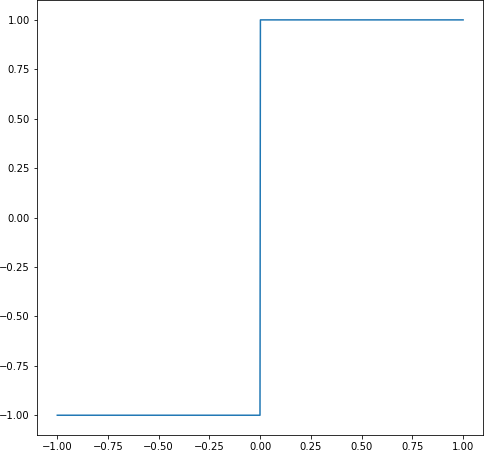
\includegraphics[width=0.4\textwidth]{Figures/sign-cropped.png}
	\caption{Traçage des fonction Signe et Heaviside}
	\label{fig:Sign-Heaviside}
\end{figure}
\FloatBarrier
\subsubsection{Binarisation décalée}
C'est une meta-binarisation qui prend une binarisation $\Psi$ et donne $\Psi$ décalé par un paramètre $\mu:$
\begin{equation}
	x\rightarrow \Psi(x+\mu)
\end{equation}
\begin{figure}[htp]
	\centering
	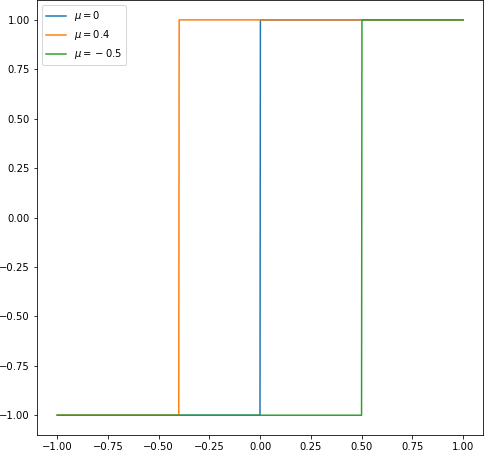
\includegraphics[width=0.33\textwidth]{Figures/shifted-sign-cropped.png}
	\caption{Traçage de la fonction signe décalée à gauche par $\mu$}
	\label{fig:ShiftedSign}
\end{figure}
\FloatBarrier
Le paramètre $\mu$ peut être fixe ou entraîné.
\subsubsection{Binarisation stochastique}
C'est aussi une meta-binarisation. Elle prend une binarisation $\Psi$ et donne $\Psi$ décalé par une variable aléatoire $z$
\begin{equation}
	x\rightarrow \Psi(x+z)
\end{equation}
\begin{figure}[htp]
	\centering
	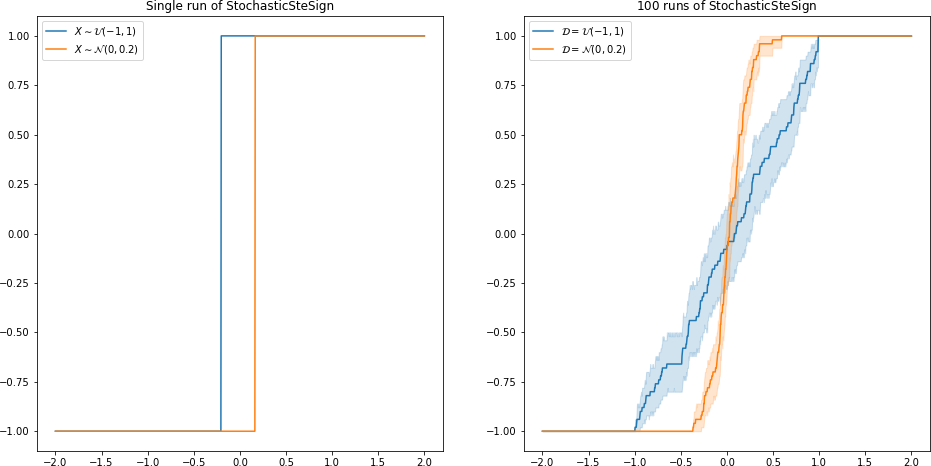
\includegraphics[width=0.66\textwidth]{Figures/stochastic-sign-cropped.png}
	\caption{Traçage de la fonction signe stochastique}
	\footnotesize
	Dans cette figure, $\mathcal{N}(0,0.2)$ dénote la distribution normale centrée avec une deviation standard $\sigma=0.2$, et $\mathcal{U}(-1,1)$ dénote la distribution uniforme dans l'interval $[-1,1]$
	\label{fig:StochasticSign}
\end{figure}
\FloatBarrier
\begin{itemize}
	
	\item La variable aléatoire $z$ suit une distribution $\mathcal{D}$ qui peut être fixe, ou même entraînée.  
	\item Cette binarisation peut être utilisé comme une forme de régularisation pour le modèle.
\end{itemize}

\newpage 
\subsection{Propagation en arrière}
On peut résumer les approximation du gradient par:
\begin{table}[h]
	\small
	\begin{tabularx}{\textwidth}{| p{3cm} | p{3cm} | X |}
		\hline
		
		Estimation & Expression & Binarisation correspende  \\
		\hline 
		STE & $\mathtt{1}_{\lvert x  \rvert} \le 1 $ &  Signe, Heavyside. \\
		\hline  
		ApproxSign & $\mathtt{1}_{\lvert x  \rvert \le 1}  \cdot (2-\lvert x \rvert) $ &  Sign\\
		\hline
		SwishSigne & $\frac{\beta \left(2-\beta x \tanh(\frac{\beta x }{2})\right)}{1+\cosh(\beta x)}$ &  Signe. \\
		\hline 
	\end{tabularx}
	\caption{Les Les estimations de gradient présentes}
\end{table}
\subsection{Implémentation}
Dans binaryflow, les binarisations sont implémentés dans le module \texttt{quantizers}
\newline Toute binarisation implémentée hérite de la classe \texttt{larq.quantizers.Quantizer}, et elle admet aussi un attribut de classe \texttt{precision} qui est égal à $1.$ 
\newline Cet attribut permet à Larq de faire les optimisations adéquates dans la phase de déploiement.
\begin{figure}[htp]
	\small
	\centering
	\begin{tikzpicture}
		\begin{abstractclass}[text width=7cm]{Quantizer}{5cm,3cm}
			\operation{call(input : Tensor[float]) : Tensor[float]}
		\end{abstractclass}
		\begin {package}{quantizers}
		\begin {class}[text width = 4.5cm]{ShiftedQuantizer}{0, 0}
		\attribute{mu : float}
		\attribute{trainable : boolean}
		\attribute{mu\_initializer : $\mathcal{R}$[float]}
		\attribute{quantizer : Quantizer}
		\inherit{Quantizer}
	\end{class}
	\begin {class}[text width = 4.5cm]{ShiftedSteSign}{0cm ,-3cm}
	\inherit{ShiftedQuantizer}
\end{class}
\begin {class}[text width = 4.5cm]{StochasticQuantizer}{5cm ,0cm}
	\attribute{distribution : $\mathcal{D}$[float]}
	\attribute{quantizer : Quantizer}
\inherit{Quantizer}
\end{class}
\begin {class}[text width = 4.5cm]{StochasticSteSign}{5cm ,-3cm}
\inherit{StochasticQuantizer}
\end{class}
\begin {class}[text width=4.5cm]{NormalSochasticSteSign}{0cm ,-5cm}
\inherit{StochasticSteSign}
\end{class}
\begin {class}[text width = 4.5cm]{UniformStochasticSteSign}{5cm ,-5cm}
\inherit{StochasticSteSign}
\end{class}
\begin {class}[text width = 2.1cm]{SteSign}{9cm ,0cm}
\inherit{Quantizer}
\end{class}
\begin {class}[text width = 2.2cm]{SteHeaviside}{11.5cm ,0cm}
\inherit{Quantizer}
\end{class}
\begin {class}[text width = 2.1cm]{ApproxSign}{9cm ,-3cm}
\inherit{Quantizer}
\end{class}
\begin {class}[text width = 2.2cm]{SwishSign}{11.5cm ,-3cm}
\inherit{Quantizer}
\end{class}
\end{package}
\end{tikzpicture}
\caption{Diagramme de classe global du module \texttt{binaryflow.quantizers}}
\end{figure}
\FloatBarrier
\newpage
\section{Régularisations}
Les BNNs supportent les régularisations offertes par les réseaux de neurones classiques.
\newline De plus, ils supportent une autre forme de régularistion appelée régularisation de quantification, qui est un terme $\mathcal{L}_{\text{quantification}}$ ajouté à la fonction objective pour réduire l'erreur de quantification:
\begin{equation}
	\mathcal{L}=\mathcal{L}_{\text{model}} + \mathcal{L}_{\text{quantification}}
\end{equation}
Le terme $\mathcal{L}_{\text{quantification}}$ comporte une somme pondérée de:
\subsection{Erreur de quantification des noeuds}
C'est égal à 
\begin{equation}
	\mathcal{L}_{\text{weight}}=\sum_{a^{(l)} \text{quantified}} \lVert \tilde{a}^{(l)} - a \rVert_p^p
\end{equation}
\subsection{Erreur de quantification des poids}
C'est égal à 
\begin{equation}
	\mathcal{L}_{\text{input}}=\sum_{\boldsymbol{W}^{(l)} \text{quantified}} \lVert \tilde{\boldsymbol{W}}^{(l)} - \boldsymbol{W}^{(l)} \rVert_p^p
\end{equation}
\subsection{Erreur de quantification de l'opération bilinéaire}
C'est aussi l'erreur de quantification de $z^{(l)}.$ 
\newline Cette erreur est l'erreur la plus importante car elle agit directement sur les performances du modèle.
\newline Elle est égale à:
\begin{equation}
	\mathcal{L}_{\text{output}}=\sum_{\boldsymbol{z}^{(l)} \text{quantified}} \left\lVert \tilde{\boldsymbol{z}}^{(l)} - \boldsymbol{z}^{(l)}  \right\rVert_p^p = \sum \left \lVert \tilde{\boldsymbol{W}}^{(l)} \star \tilde{a}^{(l-1)} - \boldsymbol{W}^{(l)} \star a^{(l-1)} \right\rVert_p^p 
\end{equation}